\chapter{Exponential integration methods in JAGUAR}

  \paragraph{}
  We want to analyse time exponential integration methods in a framework that gives us access to high-order spatial discretisation methods.
  It is possible to use high-order Finite Volume methods, but this means to use larger stensils which hurts parallelism.
  In CEDRE, users often stop at second-order methods, so we need to use an other solver.
  As the spatial discretisation method does not plays a direct role in the time integration and the work done in this thesis, we can step out from the Finite Volume framework.
  Furthermore, using a less complex solver will also help us to try and develop new methods more easily than what we already did with CEDRE.
  This is why we decided to accomplish our analysis of exponential time integration methods with the solver JAGUAR.


  \section{JAGUAR: a spectral difference solver}

    \paragraph{}
    JAGUAR means proJect of an Aerodynamic solver using General Unstructured grids And high ordeR schemes.
    It is a reactive Navier--Stokes solver originally developed at the European center for research and advanced training in scientific computing: CERFACS.
    It is made for unstructured grids, and uses a Large Eddy Simulation model to solve turbulence.
    Its particularity is that is use a spectral spatial discretisation method: the Spectral Difference method.


    \subsection{The Spectral Difference method}

      \paragraph{}
      With the Spectral Difference method, the solution is represented by a polynomial of degree $p$ inside each cell.
      It means that in the partial differential equation
      \begin{equation}\label{eq:pde_2}
        \frac{\partial u}{\partial t} + \nabla \cdot F\left(u\right) = 0 \ ,
      \end{equation}
      $u$ is a $p$-degree polynomial of the coordinate variables, where the polynomial coefficients are functions of time.
      Then $F\left(u\right)$ has to be a $p\!+\!1$-order polynomial of the coordinate variables.
      The key to the Spectral Difference method is how to compute a $p + 1$-order $F\left(u\right)$ from a $p$-order $u$.
      This method uses key elements that were first mentioned by \cite{Kopriva1996}, and was later developed by \cite{LiuVinokurWang2006}.

      \begin{figure}
        \centering
        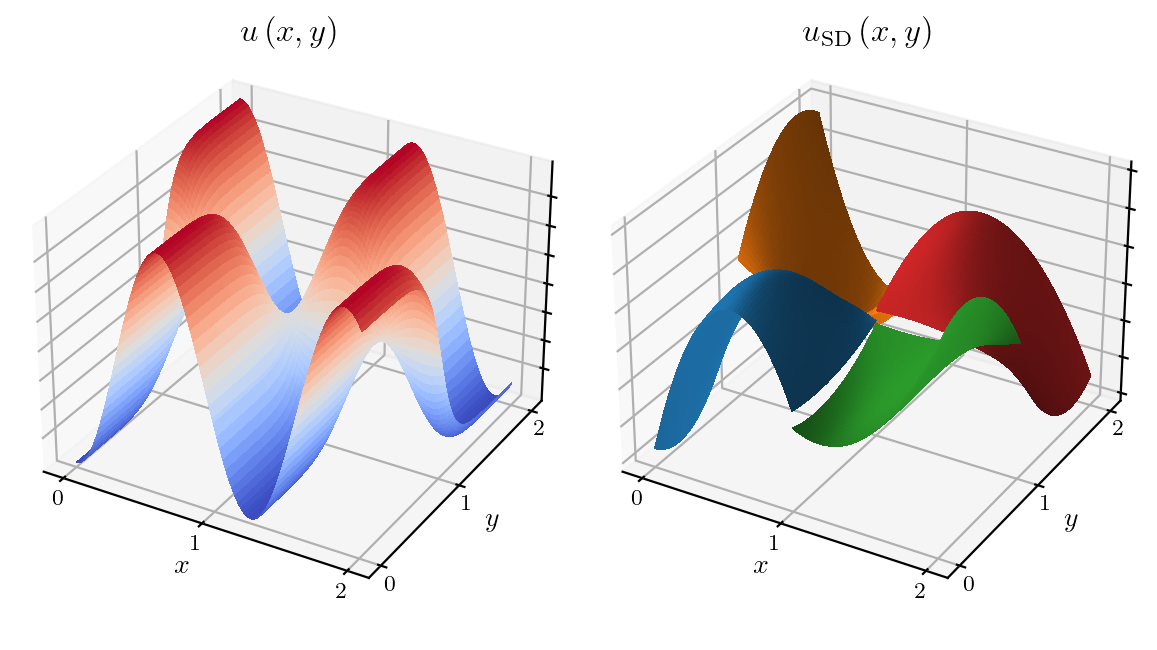
\includegraphics[width=\textwidth]{figures/sd_discontinuous.png}
        \caption{Continuous function (left) and discontinuous representation made by the Spectral Difference method (right).}
        \label{fig:sd_discontinuous}
      \end{figure}

      \paragraph{}
      Because the solution is represented in each cell by a polynomial, there is no reason for the solution to be continuous throughout cell interfaces.
      Indeed, the Spectral Difference method uses a piecewise representation of the solution.
      For example, we show in figure \ref{fig:sd_discontinuous} a function represented as the Spectral Difference method represents the solution.
      The 2D mesh is regular and made of $2 \times 2$ cells over $\left[0, 2\right]^2$.
      We represent the function
      \begin{equation}
        \begin{aligned}
          u \colon \left[0, 2\right]^2 &\to \mathbb{R}\\
          \left(x, y\right) &\mapsto \cos\left(5x\right) \tanh\left(5\left(1 - y\right)\right)
        \end{aligned}
      \end{equation}
      over the mesh in the left part of figure \ref{fig:sd_discontinuous}.
      The color mapping correspond to the output of the function but is not given as this function is of no particular interest, but is just an example for the point we make here.
      This function is interpolated with a second-order method using Lagrange polynomials over each cells.
      The result is shown in the right part of figure \ref{fig:sd_discontinuous}, where each color correspond to one cell.
      We see that there are discontinuities at the cells interfaces, and it shows a specificity of the Spectral Difference methods.
      If we were to use the function on the left part of figure \ref{fig:sd_discontinuous} as an initial condition for a simulation, the Spectral difference method would in fact use the function on the right part of the figure.
      However, to respect the underlying conservation property of equation (\ref{eq:pde_2}), it is necessary for $F$ to be continuous over the whole computational domain.
      The Spectral Difference method will them make sure that the polynomial representations of the flux density is continuous throughout cell interfaces.

      \paragraph{}
      To better understand how this method works, we take a 1D cell: the segment $\left[0, 1\right]$.
      Because the following is done at a fixed time we will drop the dependency on the time, but the solution and the coefficients are in reality functions of the time, not scalars.
      The solution $u$ inside this segment is then $u\left(x\right) = \sum_{i=0}^p a_ix^i$.
      Using Lagrange interpolation polynomials, it is equivalent to use the set of the $p + 1$ coefficients $a_i$ or the set of the $p + 1$ values $u\left(x_i\right)$ computed at the distincts points $x_i \in \left[0, 1\right]$ called \emph{solution points}.
      The solution as a $p$-order polynomial is represented by either one of those two sets.
      As the flux density $F$ must be a $p\!+\!1$-order polynomial, it can also be represented by its values in the $p + 2$ distincts \emph{flux points}.
      To ensure that $F$ is continuous at the segment end points, we take $0$ and $1$ as flux points.
      The choice of the rest of the flux points will be discussed later, but let us say for now that they are staggered with the solution points: each flux point, apart from the segment end points, is between two solutions points and vice versa.

      \begin{figure}
        \centering
        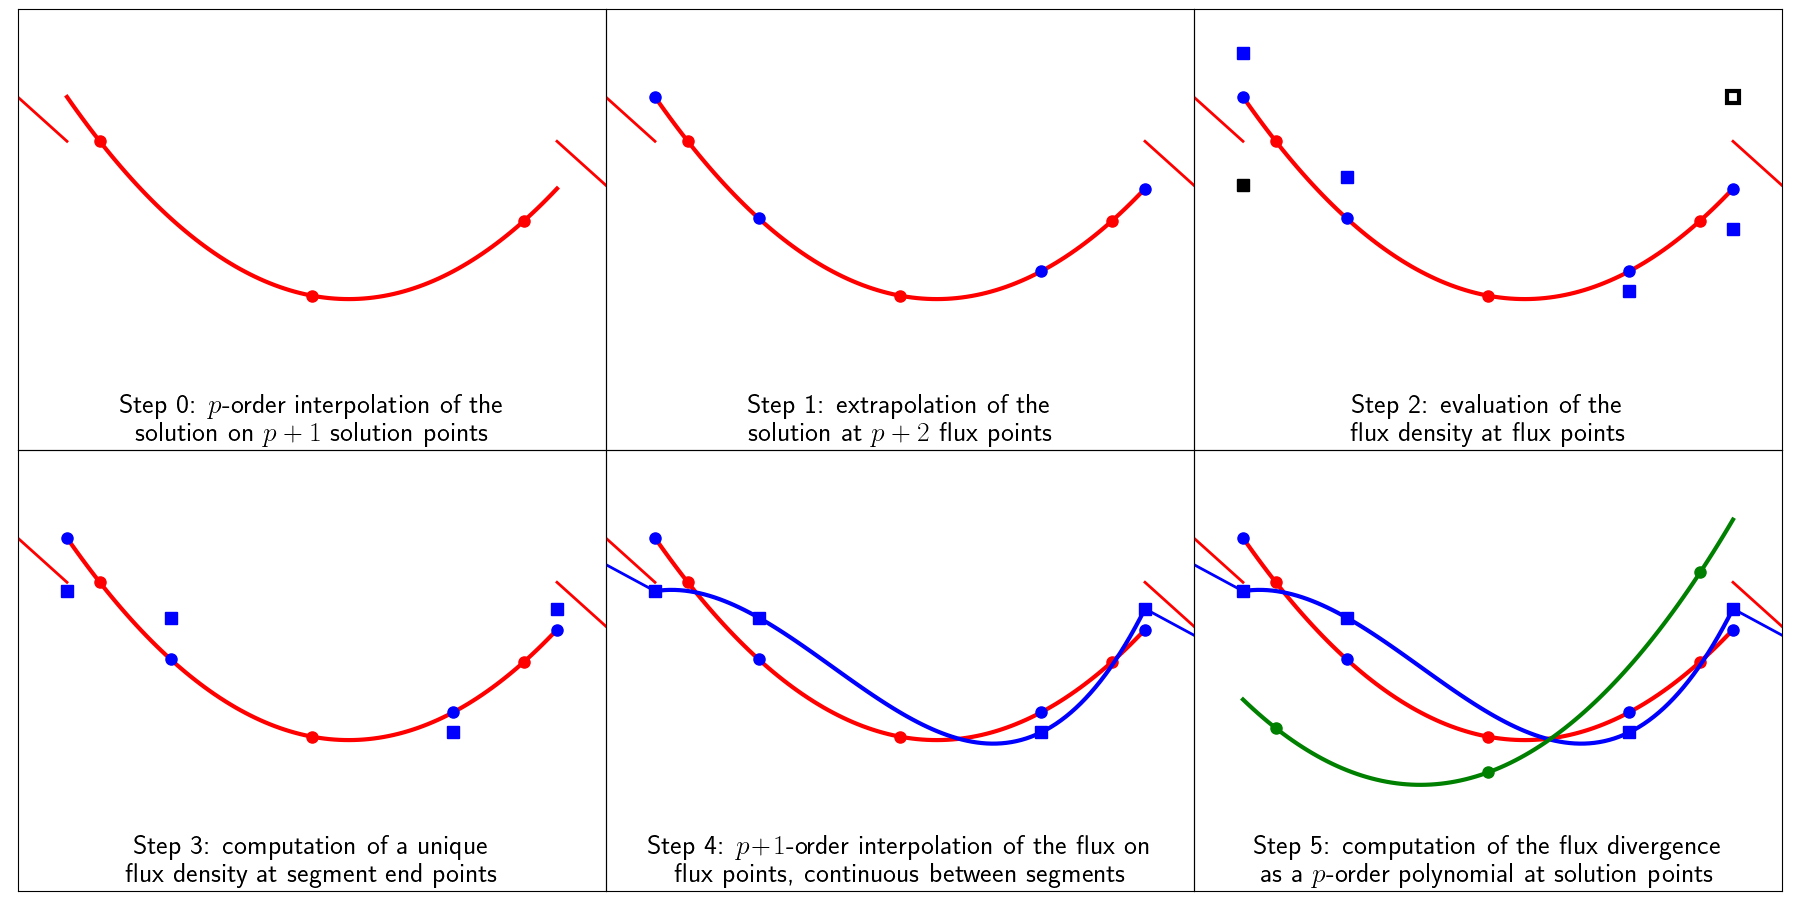
\includegraphics[width=\textwidth]{figures/sd_scheme.png}
        \caption{Steps of the Spectral Difference methods with $p = 2$.}
        \label{fig:sd_scheme}
      \end{figure}

      \paragraph{}
      Figure \ref{fig:sd_scheme} shows the steps the Spectral Difference make to compute the flux divergence $\nabla \cdot F\left(u\right)$ from the solution $u$.
      In this example, we have $p = 2$.
      \begin{enumerate}
        \setcounter{enumi}{-1}
        \item At first, the solution is represented with a red line by its value in the $p + 1$ solution points.
        The solution points are marked by red dots.
        We see parts of the solution from the left and right neighboring cells.
        As the figure shows and as we discussed before, they may be discontinuous from the solution in this cell.
        This is the starting point of the Spectral Difference method so we will call it the 0-th step.
        \item In the first step, the method computes the value of the solution in the $p + 2$ flux points, marked by blue dots.
        As the polynomial representing the solution is known, this step just consists in evaluating in at flux points.
        \item In the second step, the method evaluates the flux density $F\left(u\right)$ in each flux points.
        This is possible because we computed the solution in those points in the previous step.
        The values of the flux density are marked by blue squares in the figure.
        However, segment end points are flux points for the two neighboring cells, and therefore we show in the figure a full black square for the flux at $0$ from the left neighboring cell and an empty black square for the flux at $1$ from the right neighboring cell.
        \item Because there are different values of the flux density at the segment end points, the method would not preserve the conservative property of the partial differential equation.
        This is why in the third step, the method compute a unique interface flux density for both cell at each segment end points.
        The problem is to find the interface flux at the discontinuity of a piecewise solution.
        In other words, this is a Riemann problem.
        Once again, this is solved with a Riemann solver, exact or approximate, to get in the end a single value for the left and right parts of the discontinuity.
        \item Now that we have the value of the flux density at the $p+2$ flux points, we can interpolate it with Lagrange polynomials to get a $p+1$ order $F$ as expected in the fourth step, represented with a blue line in the figure.
        We end up with a continuous representation of $F$, differentiable everywhere except at cell interfaces.
        \item In the last step, we can differentiate the representation of $F$ to get the flux divergence, represented by a green line in the figure.
        We finally get a $p$-order representation of $\nabla \cdot F$ that we can evaluate at the solution points.
      \end{enumerate}

      \paragraph{}
      To work with any segment, not only $\left[0, 1\right]$, we use an isoparametric transformation to get back to this unity segment.
      It is the same when working with multiple dimensions, where we go back to tensors powers of this segment.
      The placement of the solution points does not seem to matter much, but the placement of the flux points does \cite{VandenAbeeleLacorWang2008}.
      The $p + 1$ solution points we will use are defined in the $\left[0, 1\right]$ segment as the Chebyshev roots:
      \begin{equation}
        x_i = \frac{1}{2} \left(1 - \cos\left(\frac{2i + 1}{2p + 2} \pi\right)\right), \quad, 0 \leq i \leq p \ .
      \end{equation}
      They are traditionally defined inside the $\left[-1, 1\right]$ segment but are scaled into $\left[0, 1\right]$.
      They are the roots of the Chebyshev polynomials of the first kind, and are often used in polynomial interpolation as they tend to minimise Runge's phenomenon.
      The $p + 2$ flux points used by our methods are the $p$ roots of the $p$-th Legendre polynomials to which are added the two segment end points.
      This choice has the property that there is a flux point between each contiguous solution points.
      There is no explicit formula for the Legendre polynomial roots as there is one got the Chebyshev polynomial roots.
      Their value is taken from tables from the literature \PS{ref ?}.
      They are also defined in the $\left[-1, 1\right]$ segment and are scaled into $\left[0, 1\right]$.
      Finally, the solution and flux points can be seen in figure \ref{fig:sd_points}.

      \begin{figure}
        \centering
        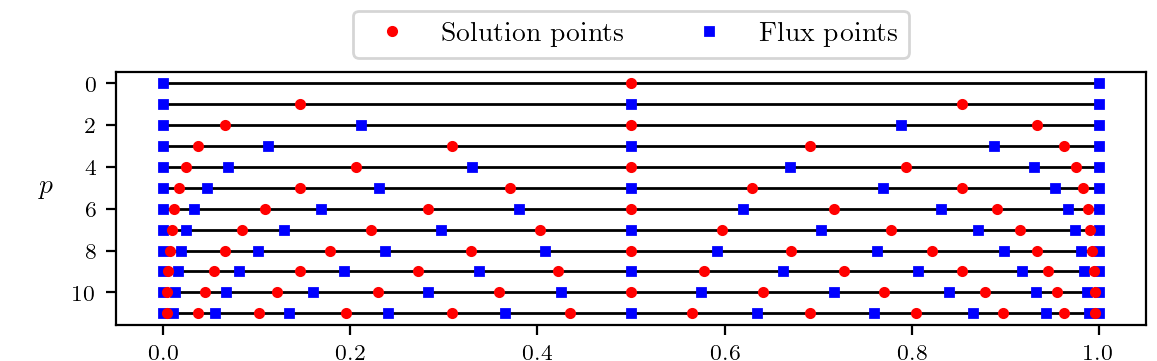
\includegraphics[width=\textwidth]{figures/sd_points.png}
        \caption{Solution points and flux points in the $\left[0, 1\right]$ segment used in the Spectral Difference method for $0 \leq p \leq 11$.}
        \label{fig:sd_points}
      \end{figure}

      \paragraph{}
      As a side note, we see that the Spectral Difference method with $p = 0$ correspond to the first-order Finite Volume method.
      Indeed, the solution is assumed constant in the cell, represented by the value at its barycenter.
      The flux balance is made at the cell interfaces with a Riemann solver.
      This correspond to the placement of the solution and flux points in figure \ref{fig:sd_points} when $p = 0$.
      For higher $p$ we have a true Spectral Difference method, of order $p$ \PS{preuve de l'ordre ?}.
      In JAGUAR, we can chose the order $p$ from 2 to 10 \PS{10 en pratique ?}.


    \subsection{Exponential integration methods in JAGUAR}

      \paragraph{}
      We now have a high-order spatial discretisation method, so that when we test our high-order time integration methods the resulting error will come mostly from the time integration and not the spatial discretisation.
      The development of an exponential time integration method was inexpensive within CEDRE as the method reuses lots of already existing parts.
      For JAGUAR that only have explicit methods, we would have to develop the Arnoldi iteration in addition to the exponential computation functions.
      As this work does not aim to produce a finely tuned method for JAGUAR but to analyse scientifically exponential methods, we decided to rely on the SLEPc library \cite{HernandezRomanVidal2005}.
      The Scalable Library for Eigenvalue Problem Computation, or SLEPc, is an extension of the software library PETSc \cite{petsc-web-page,petsc-user-ref,petsc-efficient}.
      Instead of rewriting the algorithms we need, we can use their SLEPc implementation.
      In particular, SLEPc handles what it calls \emph{Matrix Function} objects or MFN:
      \begin{quote}
        "Given a matrix $A$ and a vector $b$, the call \mintinline{c}{MFNSolve(mfn, b, x)} computes \\
        $x=f\left(A\right) b$, where $f$ is a function such as the exponential."
      \end{quote}
      As it handles the previously introduced $\varphi$-functions with its MFN objects, SLEPc is then the obvious choice of library for implementing exponential integration methods.
      Furthermore, because it relies on PETSc, it is efficiently scalable to fit our multiprocessing needs.

      \paragraph{}
      We saw that exponential methods are based on a decomposition of the ordinary differential equation such as equation (\ref{eq:ode_split}).
      However, JAGUAR uses only explicit time integration methods, so no Jacobian matrix is available.
      Computing analytically the Jacobian matrix would prove challenging as we would have to differentiate the Spectral Difference scheme, the Riemann solvers, the diffusion scheme, etc.
      It is not insurmountable, but would amount to more work than what we can afford during this thesis.
      We decided instead to reuse the work from the previous part: the Jacobian matrix will not be formed, but its effect will be computed by a finite difference approximation.
      An other reason to work with the SLEPc library is that using a finite difference approximation is easy with it.
      More precisely, it is PETSc that handles this approximation.
      To sum up, to compute $\varphi_k\left(L\right)b$ that is required for our exponential methods with $L = f'\left(y\right)$, we first use the fact that $L$ is a Jacobian matrix to create it with the appropriate PETSc data type.
      We only need to indicate to PETSc what function $L$ it is the Jacobian matrix of: $f$.
      Then, after setting the MFN object of SLEPc, we can compute the desired result.
      The Arnoldi iteration, the Scaling and Squaring algorithm and the exponential evaluation are all handled internally by the library.
      Overall, this procedure is extremely simple from our perspective and require only few lines of code to implement.
      This highlight the relevance of using the SLEPc library.

      \paragraph{}
      With what we described, we are able to write an exponential time integration method in JAGUAR.
      Other people that also work with JAGUAR did develop implicit time integration methods using PETSc.
      To continue in this direction, we decided to add a time integration method based on the generic PETSc Time Stepper \cite{AbhyankarBrownConstantinescuEtAl2018}.
      This way, a user may use most methods from PETSc in JAGUAR with no additional developments
      It includes any explicit and implicit time integration methods, but also nonlinear solvers such as Newton's methods with various line searches algorithms, linear solvers with various Krylov subspace methods and finally various preconditioning.
      However, this generic PETSc Time Stepper method was added on the side of this thesis, and therefore will not be discussed here, along with the previous work on implicit methods.


    \paragraph{}
    In the end, we now have a high-order spatial discretisation method with the Spectral Difference method that allows us to analyse and compare exponential methods.
    In the following, we will work with the three methods we developed in JAGUAR and we presented earlier in table \ref{tab:exp_rb_butcher}: the Rosenbrock--Euler, ExpRB32 and ExpRB42 methods.


  \section{Analysis of exponential time integration methods}

    \subsection{Order: convected inviscid isentropic vortex}
    \subsection{Robustness: Taylor--Green vortex}
    \subsection{Industrial application: LS89}
